\documentclass[answers]{exam} % Clase para exámenes con respuestas
\usepackage[english,spanish]{babel} % Soporte para inglés y español
\usepackage[autostyle]{csquotes} % Manejo de citas
\usepackage{amsmath, amssymb} % Paquetes para matemáticas avanzadas
\usepackage{graphicx} % Inclusión de gráficos
\usepackage{enumitem} % Personalización de listas enumeradas
% \usepackage[letterpaper,top=2cm,bottom=2cm,left=3cm,right=3cm,marginparwidth=1.75cm]{geometry} % Configuración de márgenes
\usepackage[colorlinks=true, allcolors=blue]{hyperref} % Enlaces con color

\renewcommand{\solutiontitle}{\noindent\textbf{Respuesta:}\par\noindent} % Personalización del título de respuestas
\renewcommand{\familydefault}{\sfdefault}

\pagestyle{headandfoot}
\firstpageheader{}{}{} 
\runningheader{}{}{}
\firstpagefooter{}{}{}
\runningfooter{}{}{}

\begin{document}

\large\textbf{Funciones:}
\[
	f(x)=\frac{3-\sqrt{x^2-7}}{x-4} \text{ si } x \rightarrow 4
\]\\[1em]
\[
	g(x)=\frac{x^2-9}{x(x^2+1)} \text{ si } x \rightarrow 3 \text{ y si } x \rightarrow \infty
\]\\[1em]
\[
	h(x) =
	\begin{cases}
		\dfrac{x^2 - 7x + 6}{x^2 + 5x - 6}, & \text{si } x \leq 1 \\
		\\
		\dfrac{x^3 - 1}{x^2 - 1},           & \text{si } x > 1
	\end{cases}
	\text{ , si } x \rightarrow 1
\]

\vspace{1cm}
\large\textbf{Procedimiento:}\\

\begin{questions}

	% Question 1
	\question \large\textbf{Para la primera función f(x) encontrar matemáticamente, el límite indicado.}
	\begin{solution}
		Primero, simplificamos la función. Podemos multiplicar el numerador y el denominador por el conjugado del numerador:

		\[
			f(x) = \frac{(3 - \sqrt{x^2 - 7})(3 + \sqrt{x^2 - 7})}{(x - 4)(3 + \sqrt{x^2 - 7})}
		\]

		\[
			f(x) = \frac{9 - (x^2 - 7)}{(x - 4)(3 + \sqrt{x^2 - 7})}
		\]

		Simplificando el numerador:

		\[
			f(x) = \frac{9 - x^2 + 7}{(x - 4)(3 + \sqrt{x^2 - 7})} = \frac{16 - x^2}{(x - 4)(3 + \sqrt{x^2 - 7})}
		\]

		Notamos que \( 16 - x^2 \) se puede factorizar como \( (4 - x)(4 + x) \):

		\[
			f(x) = \frac{(4 - x)(4 + x)}{(x - 4)(3 + \sqrt{x^2 - 7})}
		\]


		\[
			f(x) = \frac{-(x - 4)(4 + x)}{(x - 4)(3 + \sqrt{x^2 - 7})}
		\]


		\[
			f(x) = \frac{-(4 + x)}{3 + \sqrt{x^2 - 7}}
		\]

		Ahora, evaluamos el límite cuando \( x \rightarrow 4 \):

		\[
			\lim_{{x \to 4}} f(x) = \frac{-(4 + 4)}{3 + \sqrt{4^2 - 7}} = \frac{-8}{3 + \sqrt{9}} = \frac{-8}{3 + 3} = \frac{-8}{6} = -\frac{4}{3}
		\]

		Por lo tanto, el límite de la función cuando \( x \rightarrow 4 \) es \( -\frac{4}{3} \).

	\end{solution}

	\vspace{0.5cm}
	% Question 2
	\question \large\textbf{Usando el GeoGebra graficar la primera función, e imprimir en una escala adecuada
		(visible).}

	\begin{minipage}{\textwidth}
		\centering
		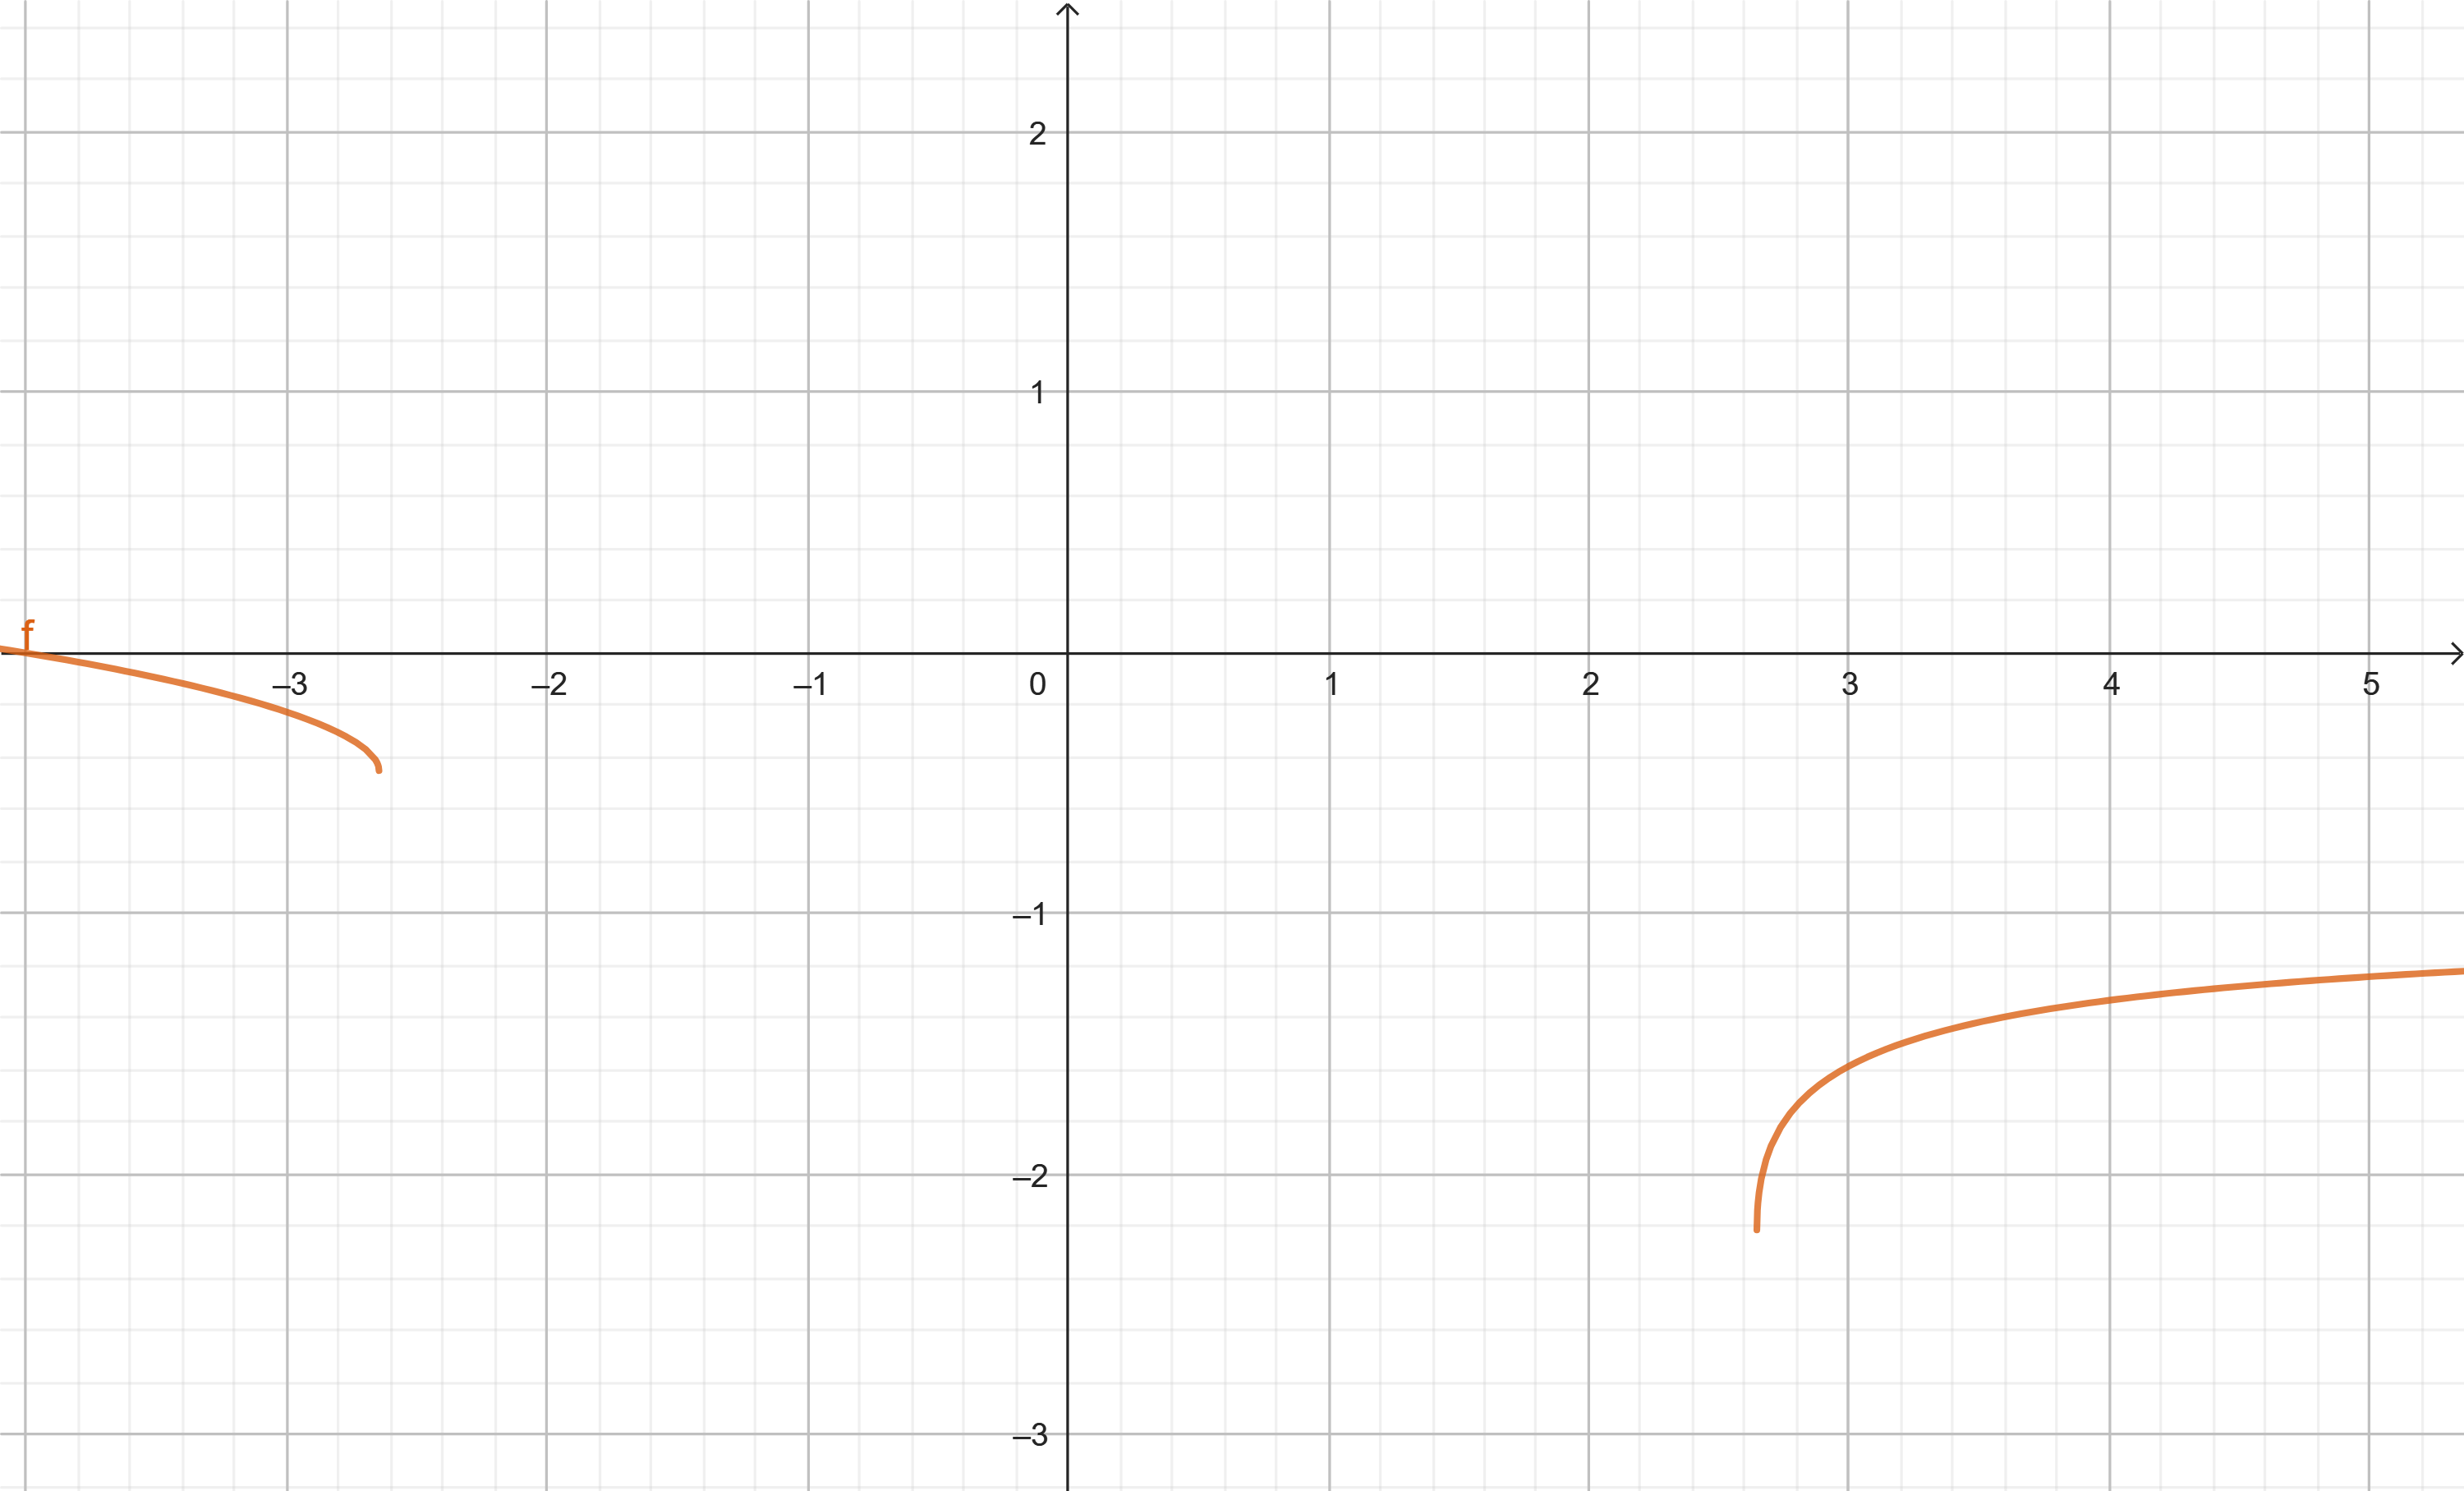
\includegraphics[width=0.9\textwidth]{public/g1.png}\\
	\end{minipage}

	\vspace{0.5cm}
	% Question 3
	\question \large\textbf{Comprobar el resultado obtenido matemáticamente con el observado en el gráfico.}
	\begin{solution}
		Al graficar la función \( f(x) \) usando GeoGebra, se observa que conforme \( x \) se acerca a 4 desde ambos lados, la función se aproxima al valor \( -\frac{4}{3} \). Esto confirma el resultado obtenido matemáticamente.
	\end{solution}

	\vspace{0.5cm}
	% Question 4
	\question \large\textbf{Repetir los numerales 1 y 2 para la función g(x) y h(x)
		.}\\[2em]
	\large\textbf{Para g(x) encontrar matematicamente el lımite indicado.:}

	\begin{solution}
		Simplificamos: \( x^2 - 9 \) se puede factorizar como \( (x - 3)(x + 3) \):

		\[
			g(x) = \frac{(x - 3)(x + 3)}{x(x^2 + 1)}
		\]

		Evaluamos el límite cuando \( x \rightarrow 3 \):

		\[
			\lim_{{x \to 3}} g(x) = \lim_{{x \to 3}} \frac{(x - 3)(x + 3)}{x(x^2 + 1)}
		\]

		Sustituyendo \( x = 3 \):

		\[
			g(3) = \frac{(3 - 3)(3 + 3)}{3(3^2 + 1)} = \frac{0 \cdot 6}{3(9 + 1)} = \frac{0}{30} = 0
		\]

		Por lo tanto, el límite de la función cuando \( x \rightarrow 3 \) es \( 0 \).

		Ahora, evaluamos el límite cuando \( x \rightarrow \infty \):

		\[
			\lim_{{x \to \infty}} g(x) = \lim_{{x \to \infty}} \frac{x^2 - 9}{x(x^2 + 1)}
		\]

		Dividimos el numerador y el denominador por \( x^2 \):

		\[
			\lim_{{x \to \infty}} \dfrac{\dfrac{x^2}{x^2} - \dfrac{9}{x^2}}{\dfrac{x(x^2 + 1)}{x^2}} = \lim_{{x \to \infty}} \dfrac{1 - \dfrac{9}{x^2}}{x + \dfrac{1}{x}}
		\]

		Conforme \( x \) tiende a infinito, los términos $\displaystyle \dfrac{9}{x^2}$ y $\displaystyle \dfrac{1}{x}$ tienden a cero:

		\[
			\lim_{{x \to \infty}} \dfrac{1 - 0}{x + 0} = \lim_{{x \to \infty}} \dfrac{1}{x} = 0
		\]

		Por lo tanto, el límite de la función cuando \( x \rightarrow \infty \) es \( 0 \).
	\end{solution}
	\newpage
	\large\textbf{Gráfico de g(x):}\\[1em]
	\begin{minipage}{\textwidth}
		\centering
		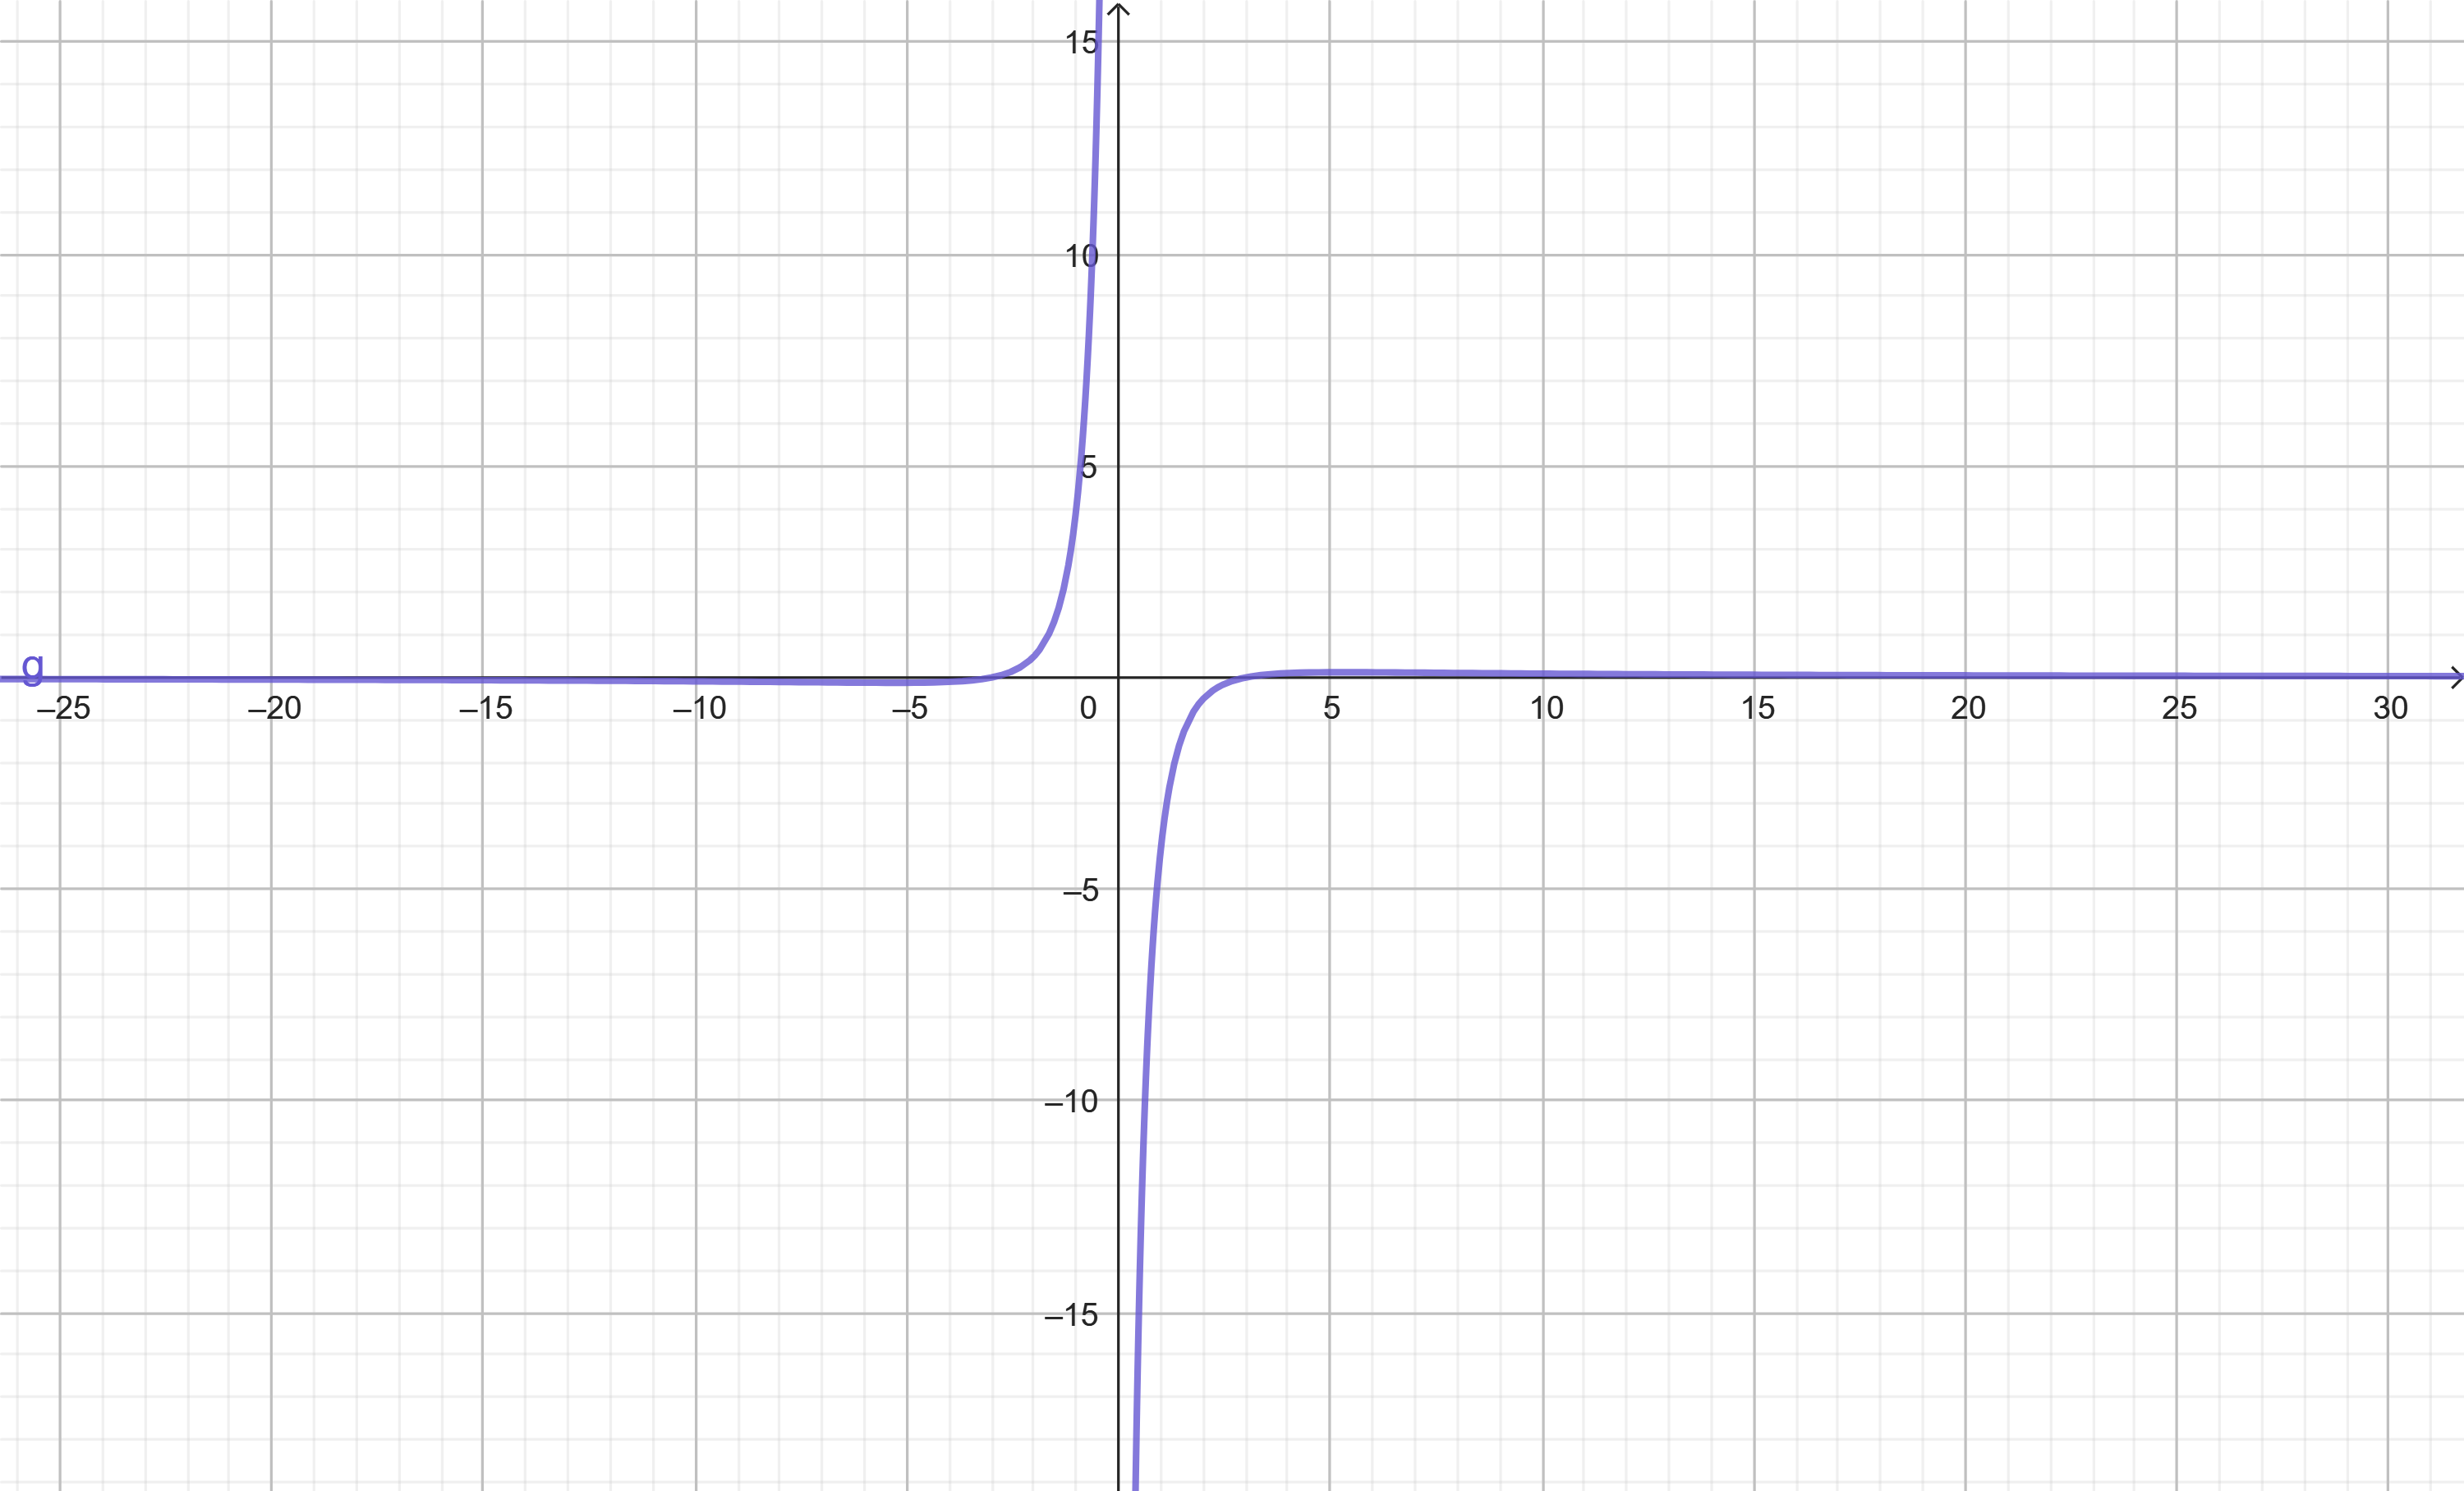
\includegraphics[width=0.9\textwidth]{public/g2.png}\\
	\end{minipage}

	\vspace{1cm}
    
	\large\textbf{Para h(x) encontrar matematicamente el lımite indicado.:}
	\begin{solution}
		La función \( h(x) \) está definida por partes:

		\[
			h(x) =
			\begin{cases}
				\dfrac{x^2 - 7x + 6}{x^2 + 5x - 6}, & \text{si } x \leq 1 \\
				\\
				\dfrac{x^3 - 1}{x^2 - 1},           & \text{si } x > 1
			\end{cases}
		\]

		Primero, evaluamos el límite cuando \( x \rightarrow 1 \) desde la izquierda (\( x \leq 1 \)):

		\[
			h(x) = \frac{x^2 - 7x + 6}{x^2 + 5x - 6}
		\]

		Factorizamos el numerador y el denominador:

		\[
			h(x) = \frac{(x - 1)(x - 6)}{(x - 1)(x + 6)}
		\]


		\[
			h(x) = \frac{x - 6}{x + 6}
		\]

		Evaluamos el límite cuando \( x \rightarrow 1 \) desde la izquierda:

		\[
			\lim_{{x \to 1^-}} h(x) = \frac{1 - 6}{1 + 6} = \frac{-5}{7} = -\frac{5}{7}
		\]

		Ahora, evaluamos el límite cuando \( x \rightarrow 1 \) desde la derecha (\( x > 1 \)):

		\[
			h(x) = \frac{x^3 - 1}{x^2 - 1}
		\]

		Factorizamos el numerador y el denominador:

		\[
			h(x) = \frac{(x - 1)(x^2 + x + 1)}{(x - 1)(x + 1)}
		\]

		\[
			h(x) = \frac{x^2 + x + 1}{x + 1}
		\]

		Evaluamos el límite cuando \( x \rightarrow 1 \) desde la derecha:

		\[
			\lim_{{x \to 1^+}} h(x) = \frac{1^2 + 1 + 1}{1 + 1} = \frac{3}{2} = \frac{3}{2}
		\]

		Como los límites laterales no son iguales, el límite de \( h(x) \) cuando \( x \rightarrow 1 \) no existe.
	\end{solution}

	\large\textbf{Gráfico de h(x):}\\[1em]
	\begin{minipage}{\textwidth}
		\centering
		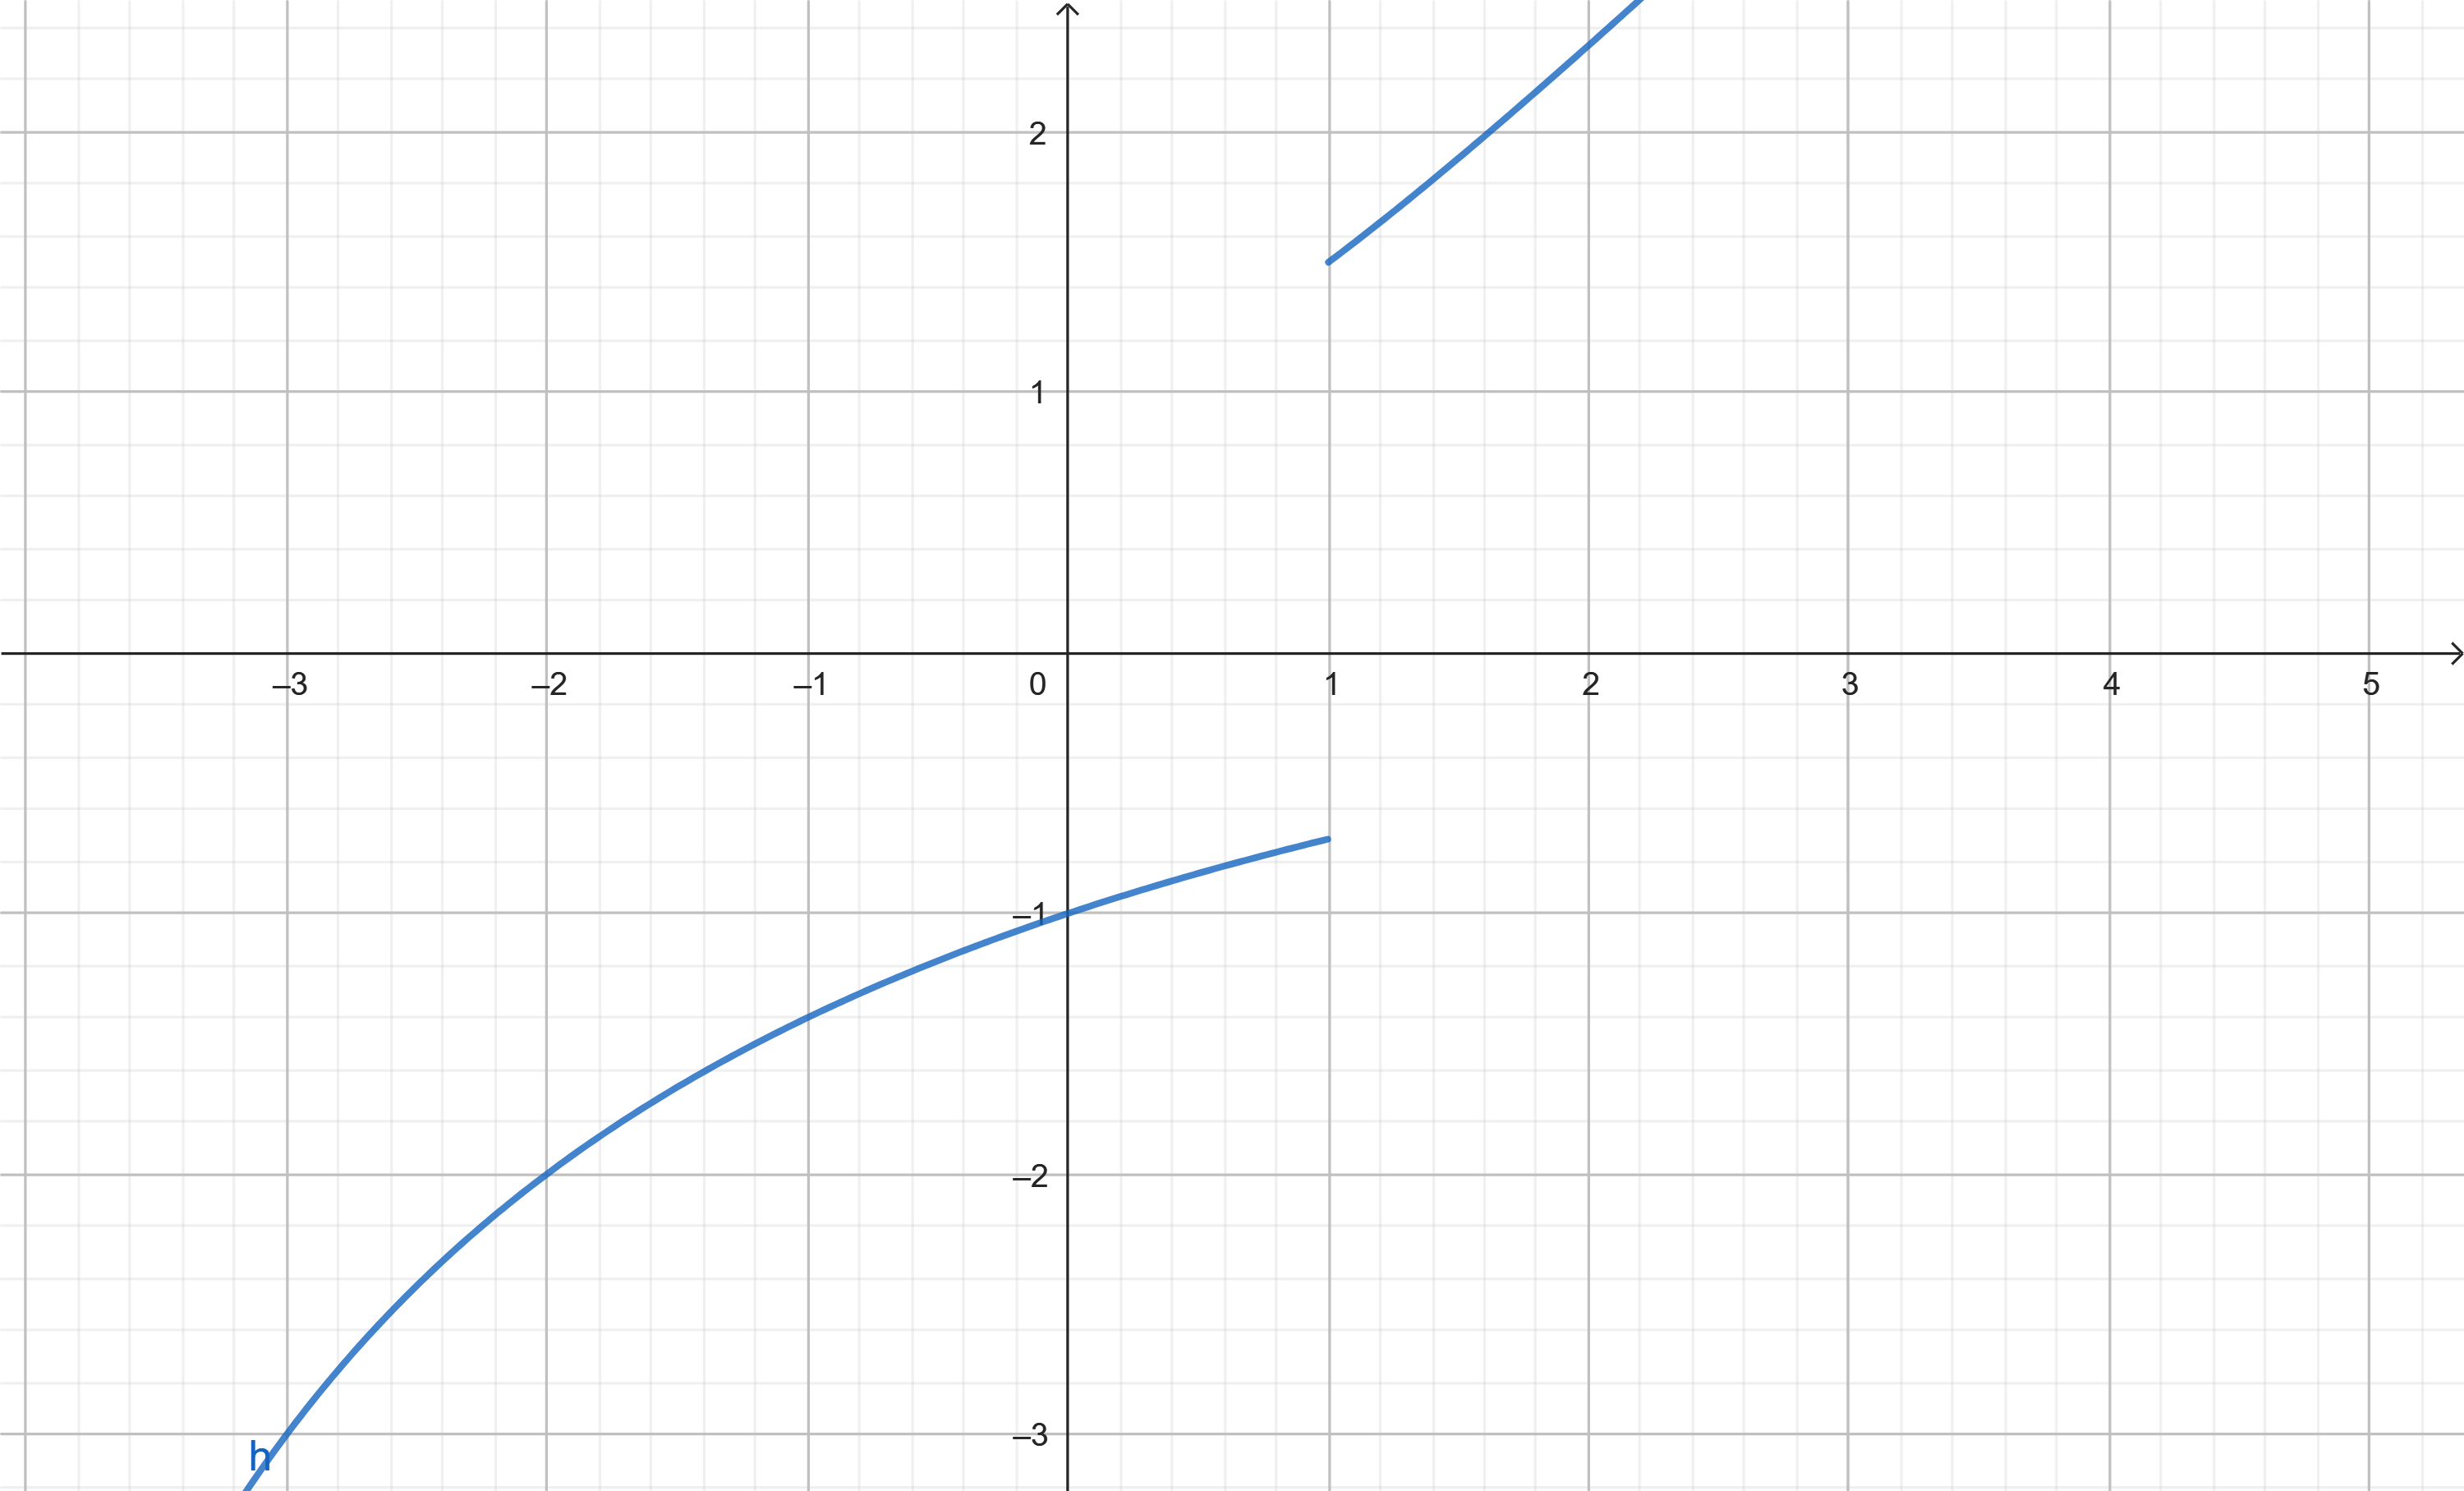
\includegraphics[width=0.9\textwidth]{public/g3.png}\\
	\end{minipage}

	\vspace{0.5cm}


\end{questions}

\end{document}
